\chapter{Arquitectura}

La aplicación sigue una variación de la arquitectura de tres capas. Las capas
de presentación y dominio permanecen inalteradas. Sin embargo, esta aplicación
no necesita de almacenamiento externo, ya que esta funcionalidad es realizada
por el servidor. Por ese motivo, la capa de persistencia ha sido sustituida por
una capa de comunicaciones.

\begin{figure}[h]
\caption{Visión general de la arquitectura}
\centering
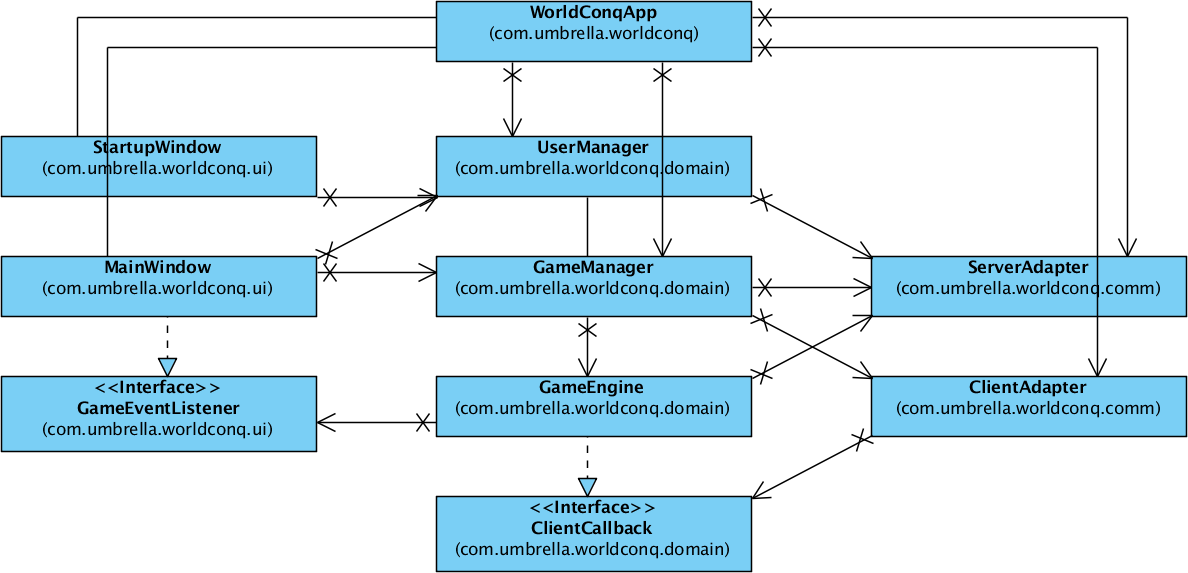
\includegraphics[width=\textwidth]{img/ch02arch-overview.png}
\end{figure}

La visibilidad entre clases va de manera jerárquica, de manera que las clases
de presentación conocen a las de dominio, y las de dominio a las de
comunicaciones, pero no al revés. Para los casos en los que es necesario un
flujo de información en sentido contrario, se han creado interfaces para
desacoplar en la medida de los posible las capas inferiores.

La clase \texttt{WorldConqApp} es la única clase que no pertenece a ninguna de
las capas. Su función es la de ser el punto de entrada de la aplicación,
encargada de crear la estructura de clases, sus relaciones, y configurarlas a
partir de los parámetros de entrada.
